\newpage
\section{Image Analysis}

When analysing images, many different approached can be taken. It all depends on which type of features needs to be extracted, and how the data looks. Based on this, the methodology can change dramatically. In this section, different methods of feature detection and extraction will be examined, as well as how to reconstruct the desired features and how to track changes in the image. The goal is to find the optimal solution for extraction of the desired features. To do this, the data needs to be examined, and easy as well as problematic frames need to be identified. 


\subsection{Problem outline} \label{imageanalysis:problemoutline}
As mentioned earlier, this project will use structured light to extract information about the object of choice. The structured light is a red laser, which has its light split into multiple smaller dots using a refracting element. These dots are the feature points that need to be extracted in the smartest way possible. To get a good understanding of the problem, some example images from different data collections must be examined. In the figures below are a few images, where some are considered "easy" and some more "difficult" to work with. The images originate from two different setups and data collections. 
Figure \ref{fig:cross1_base} and \ref{fig:cross2_base} presents the base case. Here all dots are nicely visible on a solid background. This is considered an easy frame.
\begin{figure}[h!]
    \centering
    \begin{minipage}[t]{0.48\textwidth}
        \centering
        \includegraphics[width=0.95\textwidth]{figures/ImageAnalysis/cross1_base.png}
        \caption{Collection 1, base case.}
    \label{fig:cross1_base}
    % frame number 5
    \end{minipage}%
    \hspace{.03\textwidth}
    \begin{minipage}[t]{0.48\textwidth}
        \centering
        \includegraphics[width=0.95\textwidth]{figures/ImageAnalysis/cross2_base.png}
        \caption{Collection 2, base case}
        \label{fig:cross2_base}
        % frame number 5
    \end{minipage}
\end{figure}
\FloatBarrier
In both data sets, there was glare present. This can be seen on figure \ref{fig:cross1_glare} and \ref{fig:cross2_glare}. The glare is most likely due to the camera frame and laser lining up perfectly to create a total reflection of the light from the dots, which end up hitting the camera lens directly. In this case, the dots no longer look red, but becomes fully saturated and look white instead. For the second data collection, the camera and laser were moved slightly to try to reduce the glare. It was partially successful. These are considered difficult frames.
\begin{figure}[h!]
    \centering
    \begin{minipage}[t]{0.48\textwidth}
        \centering
        \includegraphics[width=0.95\textwidth]{figures/ImageAnalysis/cross1_glare.png}
        \caption{Collection 1, more difficult case with glare.}
    \label{fig:cross1_glare}
    % frame number 171
    \end{minipage}%
    \hspace{.03\textwidth}
    \begin{minipage}[t]{0.48\textwidth}
        \centering
        \includegraphics[width=0.95\textwidth]{figures/ImageAnalysis/cross2_glare.png}
        \caption{Collection 2, more difficult case with glare.}
        \label{fig:cross2_glare}
        % frame number 346
    \end{minipage}
\end{figure}
\FloatBarrier


For both data collections, there are problems with occlusions due to the long "arms" of the cross, and the angle of the camera. This is most prominent in the first data collection as seen in figure \ref{fig:cross1_occlusion}. For the second data collection, the laser was moved slightly. This reduced the intensity of the dots, therefore become less visible. This can be seen in figure \ref{fig:cross2_low_light}. 
\begin{figure}[h!]
    \centering
    \begin{minipage}[t]{0.48\textwidth}
        \centering
        \includegraphics[width=0.95\textwidth]{figures/ImageAnalysis/cross1_occlusion.png}
        \caption{Collection 1, potentially difficult case due to occlusion.}
    \label{fig:cross1_occlusion}
    % frame number 436

    \end{minipage}%
    \hspace{.03\textwidth}
    \begin{minipage}[t]{0.48\textwidth}
        \centering
        \includegraphics[width=0.95\textwidth]{figures/ImageAnalysis/cross2_low_light.png}
        \caption{Collection 2, potentially difficult case due to very low intensity of the dots.}
        \label{fig:cross2_low_light}
        % frame number 641
    \end{minipage}
\end{figure}
\FloatBarrier
Based on this data, a few key points to base the next steps upon, can be identified. The dots are primarily red, so HSV or RGB filters could most certainly be useful. There needs to be some correction for the saturated dots when glare occurs though. 

The strongest features are the cross, and the dots. The dots are even stronger compared to the cross for the second data collection. The possibility of blurring the images and subtracting them from the original frames to create masks of features will be explored.

Some of the dots are small, so some reconstruction using morphological operators might be necessary.

To automatically locate the dots, different algorithms for computing contours of the dots will be explored.


With these considerations in mind, the following methods will be explored:\\


Three different methods to extract feature points are inspected:
\begin{enumerate}
    \item HSV and RGB Color Space Threshold.
	\item Canny Edge Detection.
	\item Blur and Subtract using Gaussian kernel.
\end{enumerate}

Two fundamental morphological operators are defined:
\begin{enumerate}
	\item Dilation and Erosion
	\item Closing and Opening
\end{enumerate}

Three different methods to fetch coordinates of feature points are examined:
\begin{enumerate}
	\item Contour Search.
	\item Hough Circle Transformation.
\end{enumerate}

A short section on elimination of outliers using epipolar lines and knowledge of the setup. \\

Finally, a proposed optimal solution is found and presented.\\

The frames used in the problem outline that visualize different difficulties in the data will be reused to test proposed filters. The reader is encouraged to go back to this section to see the original frames, and compare with the filtered ones. \\

Data for the image analysis was collected twice. The first and second data collection will both be used to evaluate filter performances, as this will shed more light on benefits and potential pitfalls using different methods. When we move forward to reconstruct the actual point cloud, only data collection 2 will be used, as another object was scanned using this setup. This will allow us to test the proposed solution on more than one object, to evaluate performance better. 




%image numbers for testing
% base1 = 5,          base2 = 5
% glare1 = 171,       glare2 = 346
% occlusion1 = 436,   lowlight2 = 641

\subsection{Feature Extraction}
The methods outlined in the previous section about feature extraction will be examined in detail here, starting with filtering of the image using different color spectra.




\subsubsection{Color filtering and saturation detection}
Given that the dots are mostly red, it seems obvious to try filtering using the RGB color space. This is done by thresholding the three colors using different values. Hereafter, only the desired part of the defined colors are left. The image is converted to binary, and the colors above the threshold are set to 1, and the rest is set to 0 (of course, the filter can be defined inversely too). \\
By induction, a filter for the base case from data collection 1 was created (see fig. \ref{fig:base1_no_glare_filt}). This filter works, but it cannot handle glare as can be seen in figure \ref{fig:glare1_no_glare_filt}. The main issue here is that the images with glare contains a lot of high saturation values. The simple RGB filter only looks for red color. 
\begin{figure}[h]
    \centering
    \includegraphics[width=0.8\textwidth]{figures/ImageAnalysis/filtered_base1_noglarefilt.png}
    \caption{Collection 1. Base case RGB filter used on base image.}
    \label{fig:base1_no_glare_filt}
\end{figure}
\FloatBarrier
\begin{figure}[h]
    \centering
        \includegraphics[width=0.8\textwidth]{figures/ImageAnalysis/filtered_glare1_noglarefilt.png}
        \caption{Collection 1. Base case RGB filter used on glare image. Image is cropped to enhance detail.}
        \label{fig:glare1_no_glare_filt}
\end{figure}
\FloatBarrier
This method does not work well for data collection 2, as it also has glare issues. It is desired to create a filter that works for all data that is collected. 


A filter that is designed to extract dots when glare is present, can easily be created. This was tested, and the performance was of course good when glare was present but bad at all other times.  


To accommodate the base frames and glare, a filter in the HSV color spectrum is created.\\

The HSV color spectrum consists of hue (H), saturation (S), value (V). \texttt{Hue} is defined as a location on a wheel of color. 0 is start and 1 is end (a full rotation). The color wheel starts with red, moving to orange and green, then to magenta and blue, ending back at red. \texttt{Saturation} is on a scale from 0 to 1 and describes the amount of white light being mixed in with the color. Finally, \texttt{value} defines the maximum of red, green, and blue in the image. \\

To convert an RGB image to HSV, the following four equations are used:
\begin{equation}
    H=\left\{\begin{array}{cc}
\theta & \text { if } B \leq G \\
360-\theta & \text { if } B>G
\end{array}\right. \\
\label{eq:hue}
\end{equation}
\begin{equation}
\theta=\cos ^{-1}\left\{\frac{\frac{1}{2}[(R-G)+(R-B)]}{\left[(R-G)^{2}+(R-B)(G-B)\right]^{1 / 2}}\right\}
\end{equation}
\begin{equation}
S=1-\frac{3}{(R+G+B)}[\min (R, G, B)]
\end{equation}
\begin{equation}
    V = \text{max} \left(R,G,B \right)
\end{equation}



As mentioned, hue is a circular function and is thus described using an angle $\theta$. If the angle is defined in radians, so should the switch case in eq. \ref{eq:hue} be. \\


This spectrum is useful because the hue of the dots doesn't change, only the saturation level, at least for data collection 1. 
The filter designed for the base case of data collection 1, only allows a narrow band of colors with a red hue, cuts the first 20\% off of saturation, and cuts the first 65\% off of value. The filter works nicely and extracts the dots. For the glare case, it doesn't work well, as seen in figure \ref{fig:glare1_no_glare_filt_hsv}. \\

A different filter was designed for the case with glare, and then dots are extracted nicely when there is glare in the image as seen in figure \ref{fig:glare1_glare_filt_hsv}. Though, when there is no glare, very few dots are extracted.
\begin{figure}[h!]
    \centering
    \begin{minipage}[t]{0.48\textwidth}
        \centering
        \includegraphics[width=0.95\textwidth]{figures/ImageAnalysis/filtered_glare1_noglarefilt_hsv.png}
        \caption{Collection 1. HSV Filter designed for base case used on image with glare present. Image is cropped to enhance detail. }
    \label{fig:glare1_no_glare_filt_hsv}
    \end{minipage}%
    \hspace{.03\textwidth}
    \begin{minipage}[t]{0.48\textwidth}
        \centering
        \includegraphics[width=0.95\textwidth]{figures/ImageAnalysis/filtered_glare1_glarefilt_hsv.png}
        \caption{Collection 1. HSV Filter designed for glare case used on image with glare present. Image is cropped to enhance detail}
        \label{fig:glare1_glare_filt_hsv}
    \end{minipage}
\end{figure}
\FloatBarrier


This filter also works well when glare is present for data collection 2. 
As one could expect, the primary difference between an HSV filter defined for base and glare case is the saturation scaling. \\
If one only had two filters to choose from, depending on the amount of glare in a certain frame, the dot extraction would have very poor performance. To fix this, the scaling of the saturation based on the amount of white in the image will be examined. \\

The histograms for a base case image with good lighting condition, vs. one with a lot of glare, looks similar as seen in figures \ref{fig:hist_base1} and \ref{fig:hist_glare1}. 
\begin{figure}[h!]
    \centering
    \begin{minipage}[t]{0.48\textwidth}
        \centering
        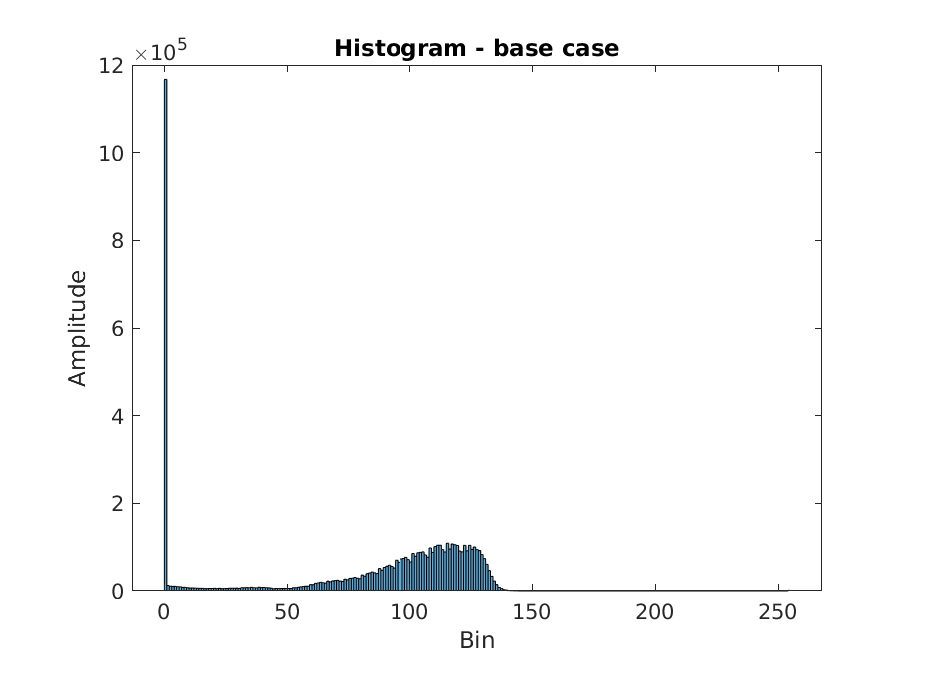
\includegraphics[width=0.95\textwidth]{figures/ImageAnalysis/Histogram_base1.eps}
        \caption{Collection 1. Histogram for base case.}
    \label{fig:hist_base1}
    \end{minipage}%
    \hspace{.03\textwidth}
    \begin{minipage}[t]{0.48\textwidth}
        \centering
        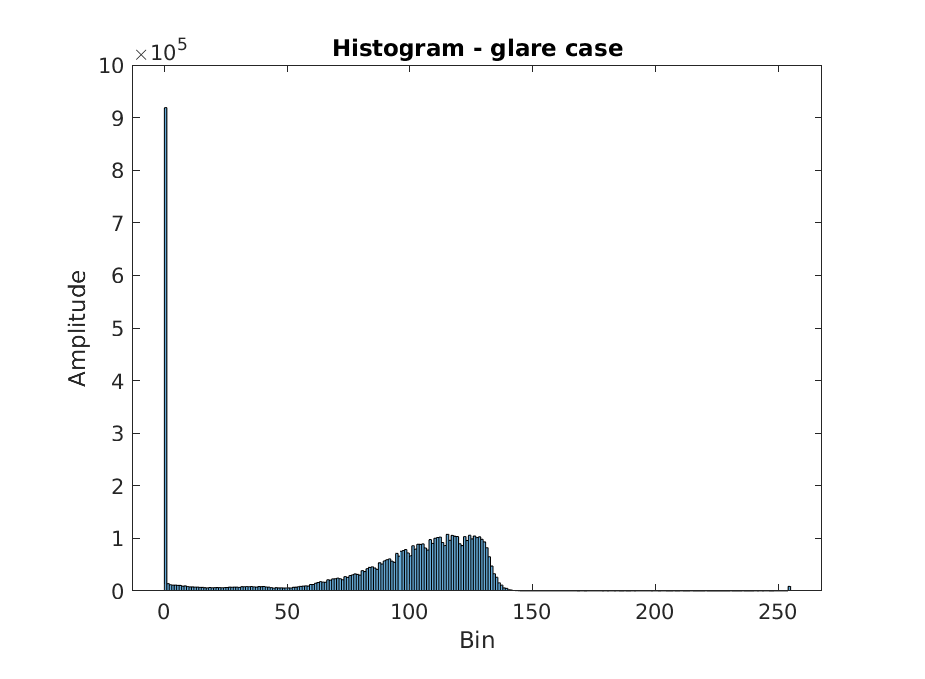
\includegraphics[width=0.95\textwidth]{figures/ImageAnalysis/Histogram_glare1.eps}
        \caption{Collection 1. Histogram for glare case}
        \label{fig:hist_glare1}
    \end{minipage}
\end{figure}
The curve of the plot is alike, but the scaling is completely different. To track the white in the images, only the last 5 bins will be considered, as these contain the relevant information. They are plotted in figure \ref{fig:hist_base1_zoom} and \ref{fig:hist_glare1_zoom}.
\begin{figure}[h!]
    \centering
    \begin{minipage}[t]{0.48\textwidth}
        \centering
        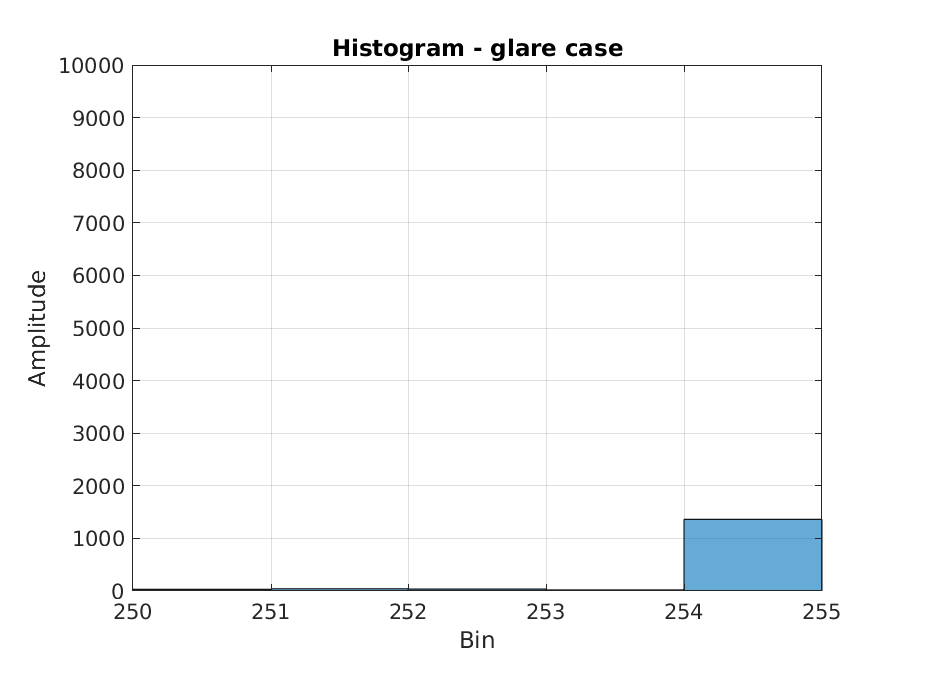
\includegraphics[width=0.95\textwidth]{figures/ImageAnalysis/Histogram_base1_zoom.eps}
        \caption{Collection 1. Histogram for base case, zoomed in on bin [250,255].}
    \label{fig:hist_base1_zoom}
    \end{minipage}%
    \hspace{.03\textwidth}
    \begin{minipage}[t]{0.48\textwidth}
        \centering
        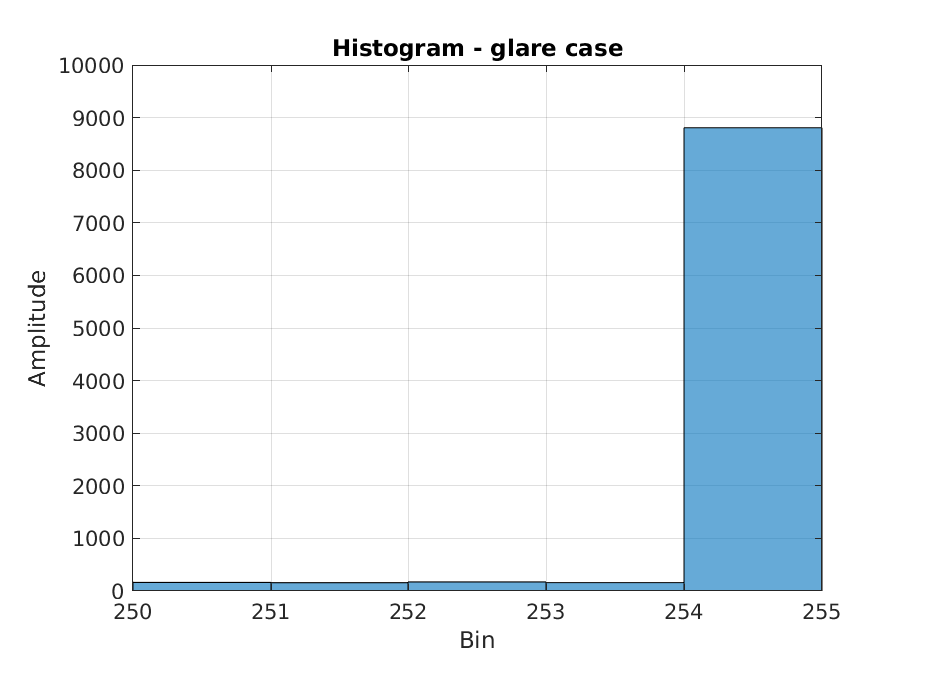
\includegraphics[width=0.95\textwidth]{figures/ImageAnalysis/Histogram_glare1_zoom.eps}
        \caption{Collection 1. Histogram for glare case, zoomed in on bin [250,255].}
        \label{fig:hist_glare1_zoom}
    \end{minipage}
\end{figure}
\FloatBarrier
Based on these histograms, it can be concluded, that it is only useful to look at the very last bin, as this contains information about saturation.\\

To utilize this fact, an HSV filter was created. The filter is made such that the upper limit for the saturation is inversely scaled with the white level of the image. When the white level is high, the saturation has a low maximum value. When the white level is low, the saturation has a high maximum value. 
This is because when glare occurs, the center of dots becomes white and saturated, but the outside of the dots bleed red light.\\


The minimum value for the upper bound saturation level is 0.4. The maximum value for the upper bound saturation level is 1. The linear mapping of the saturation can be seen in equation \ref{eq:hist_scaling}
\begin{equation}
    \text{Upper bound saturation} = 1-\frac{1-0.4}{100} \cdot \frac{cur-min}{max-min}
    \label{eq:hist_scaling}
\end{equation}
$min$ and $max$ are the minimum and maximum values of bin 255 of the histogram for the entire data collection, and $cur$ is the value from bin 255 in the current image. \\

Using the same HSV filter as before, with saturation level adjusted for each image by this new mapping, the following results are retrieved (fig \ref{fig:hsv_filt_both_base}, \ref{fig:hsv_filt_both_glare})
\begin{figure}[h]
    \centering
        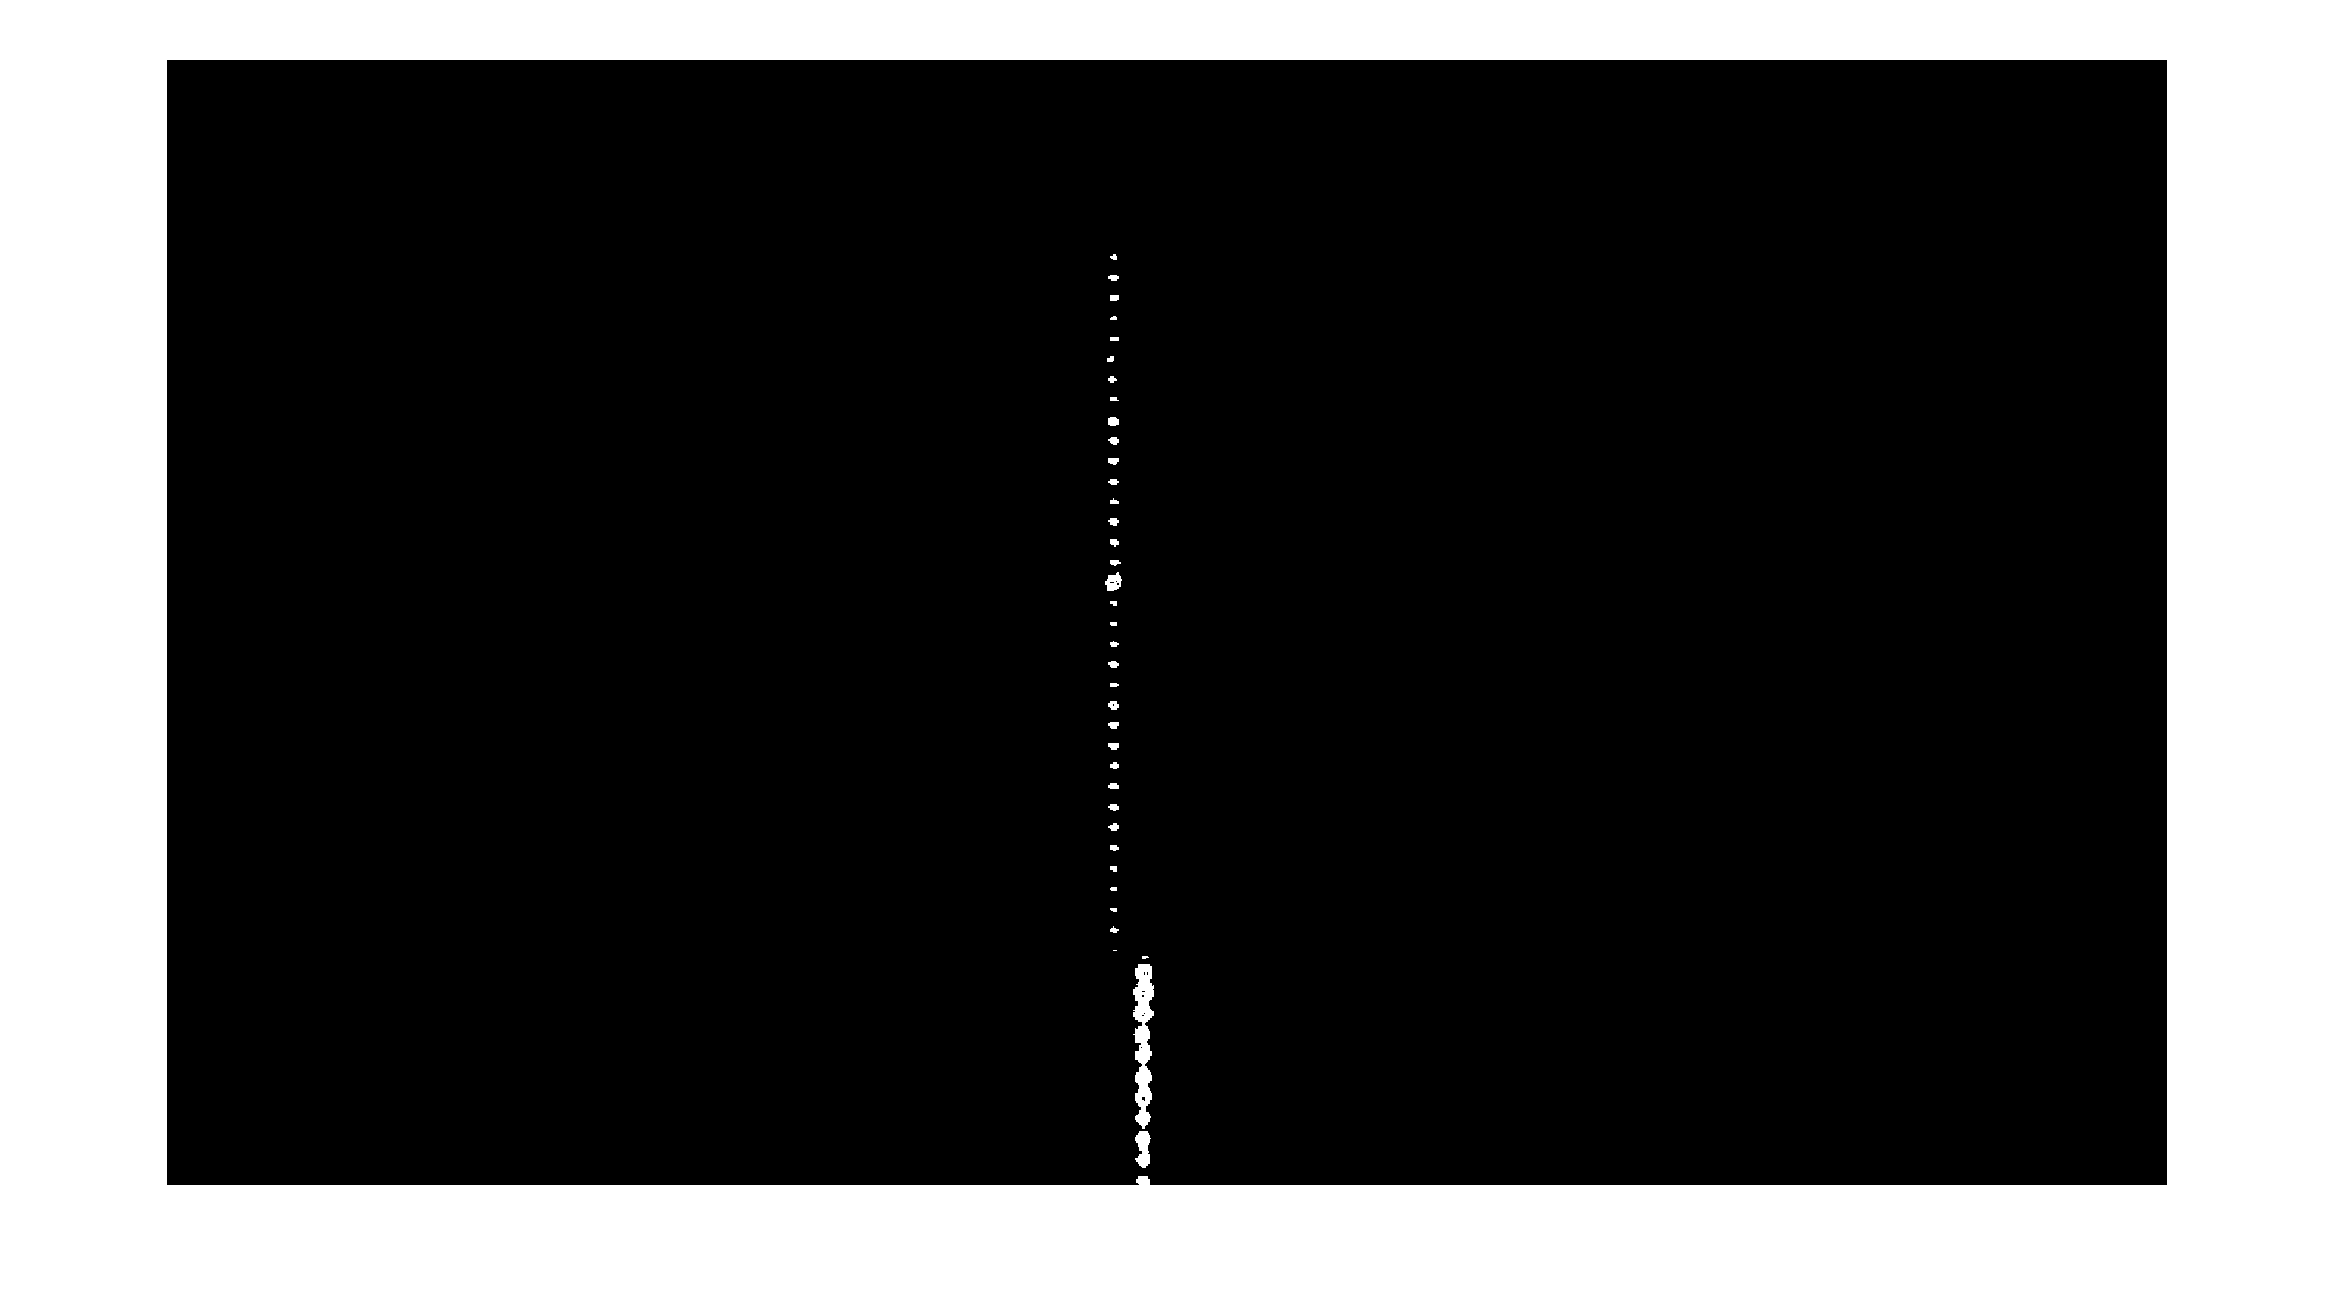
\includegraphics[width=0.95\textwidth]{figures/ImageAnalysis/filtered_base1_hsv_both.eps}
        \caption{Collection 1. Single HSV filter with linear mapping of saturation used on base frame.}
    \label{fig:hsv_filt_both_base}
\end{figure}
\begin{figure}[h]
\centering
    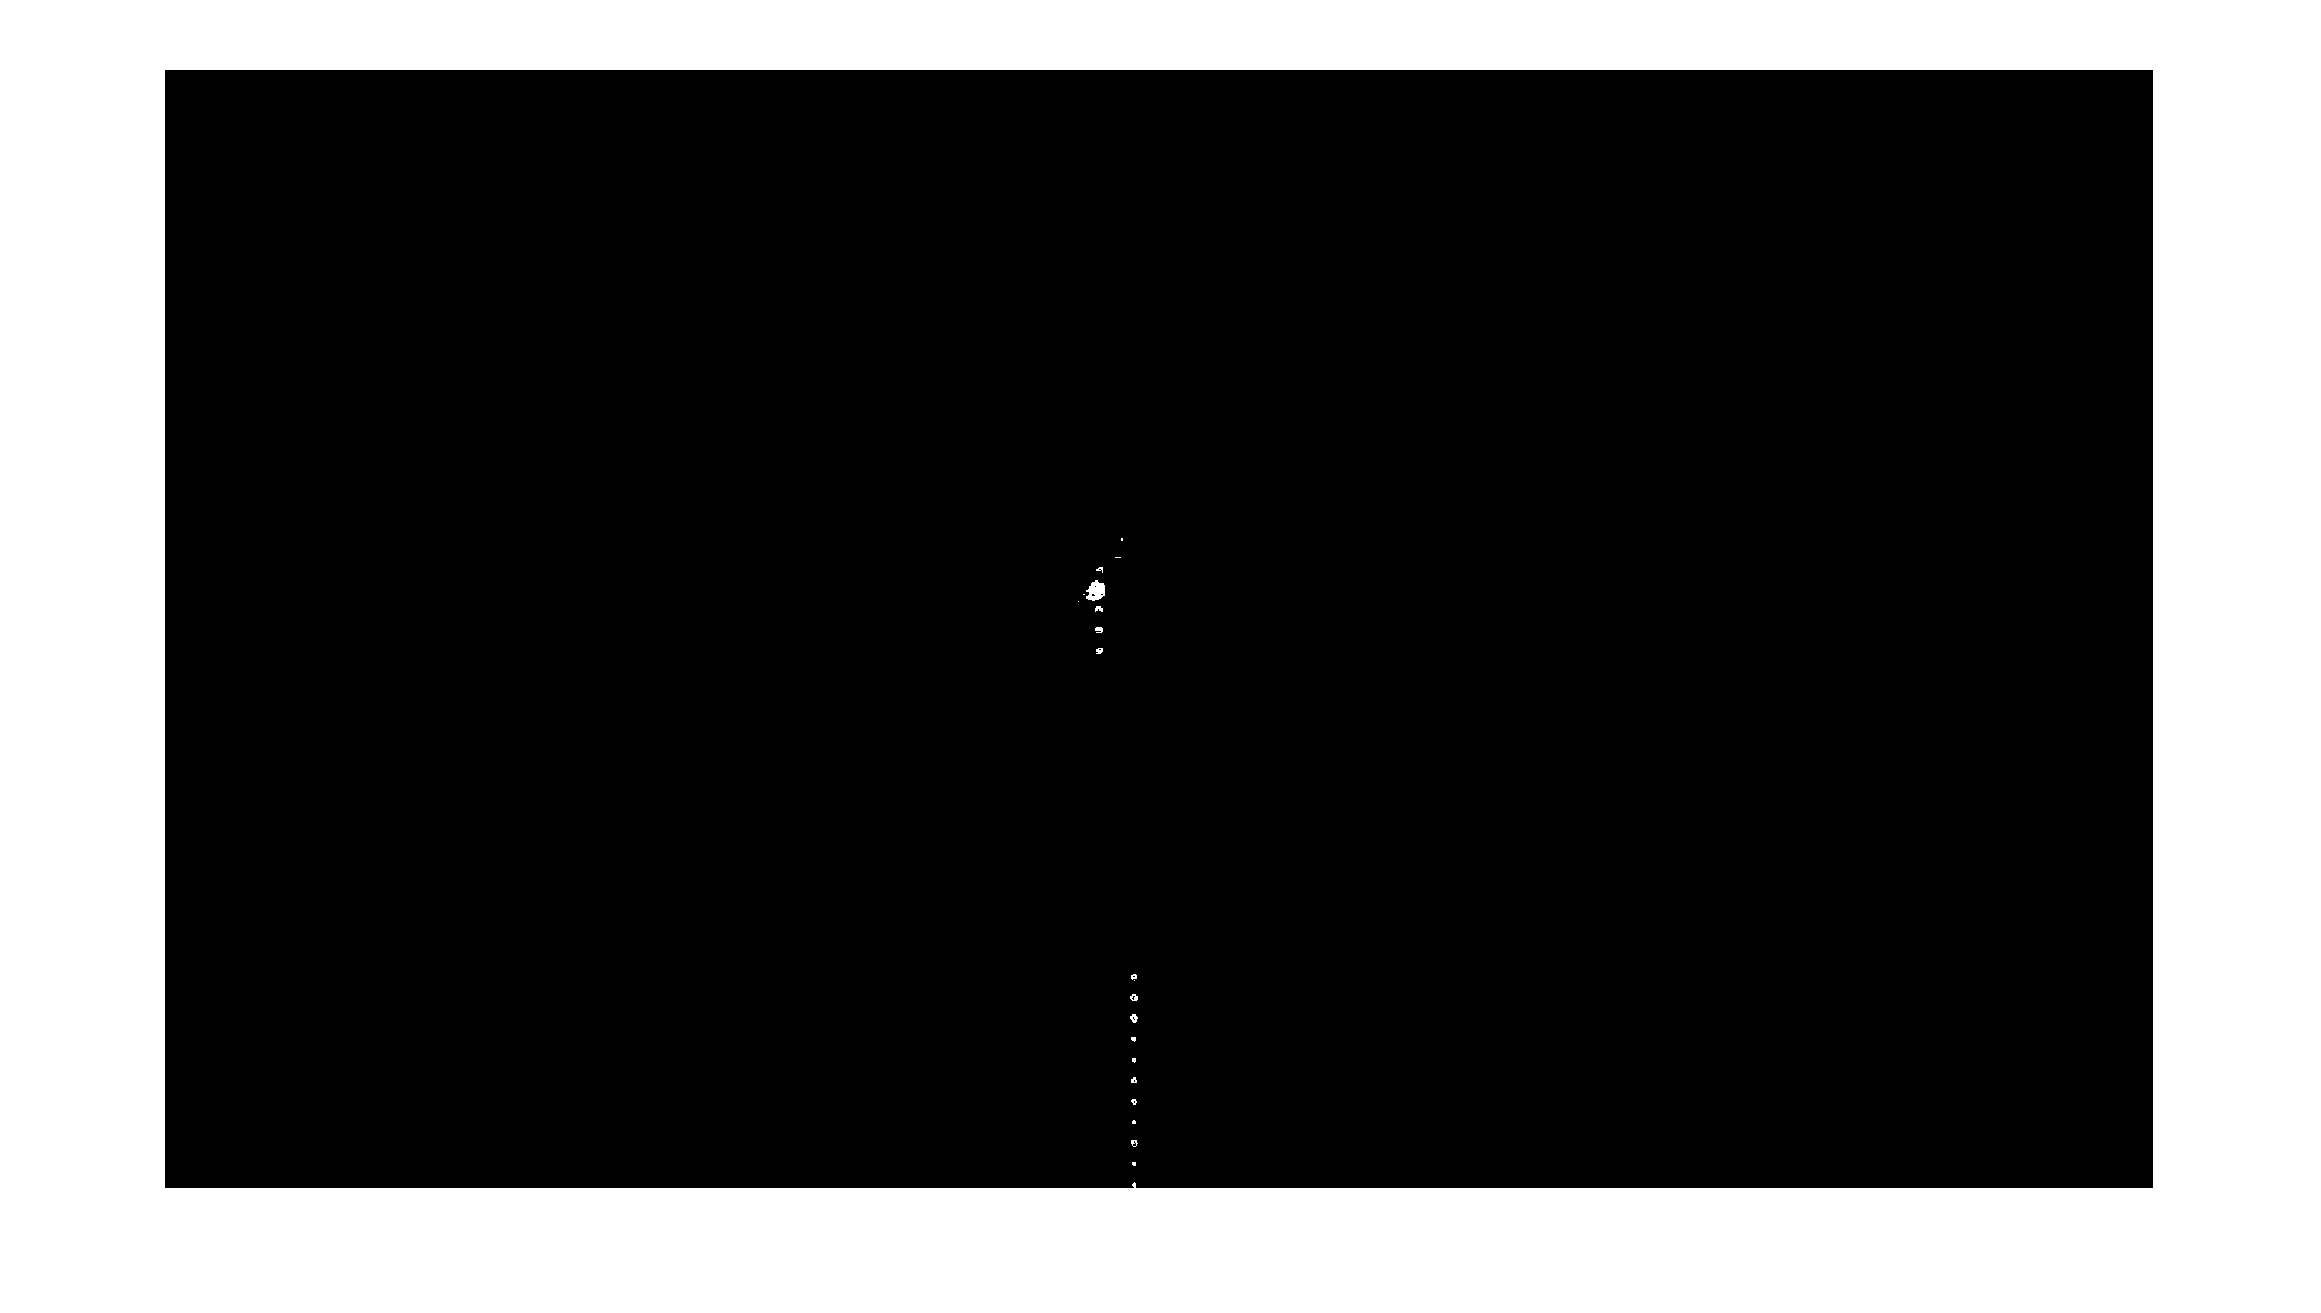
\includegraphics[width=0.95\textwidth]{figures/ImageAnalysis/filtered_glare1_hsv_both.eps}
        \caption{Collection 1. Single HSV filter with linear mapping of saturation used on frame with glare.}
        \label{fig:hsv_filt_both_glare}
\end{figure}
\FloatBarrier
The dots are extracted to satisfying degree, but can we do better? This filter works for the data collection, and also somewhat for data collection 2, but might not be that robust in general. Furthermore, this filter needs to traverse through the entire image first to find minimum and maximum saturation values, or do this manually, before you can start extracting dots. This is computationally not smart. To improve upon this, other methods will be examined in the following section. 


% [1] Chapter 10.2, page 710
% [2] Chapter 10.2, page 716
% [3] Chapter 10.2, page 732
% [4] Chapter 10.2, page 729
% [5] Chapter 10.2, page 730

% https://docs.opencv.org/3.4/d7/de1/tutorial_js_canny.html
% https://docs.opencv.org/3.4/da/d5c/tutorial_canny_detector.html 
	
\subsubsection{Canny Edge Detection}
Edge detection is an approach used frequently for segmenting images based on abrupt changes in intensity. This can be accomplished using first or second order derivatives.  In order to detect changes in intensity, one has to find the edge strength which is defined by 
\begin{equation}
	\nabla f(x,y) \equiv  g_x(x,y) \\ g_y(x,y) \ = \begin{bmatrix} \frac{\partial f(x,y)}{\partial x} \\ \frac{\partial f(x,y)}{\partial y} \end{bmatrix} 
\end{equation}

and the magnitude of the gradient vector at point $(x,y)$ which is given by
\begin{equation}
	M(x,y) = ||\nabla f(x,y)|| = \sqrt{g_x^2(x,y)+g_y^2(x,y)}
\end{equation}

and the direction of the gradient vector at point $(x,y)$ which is given by \cite{gonzalez2018digitalChapter10.2}
\begin{equation}
	\alpha(x,y) = \tan^{-1}\left[\frac{g_y(x,y)}{g_x(x,y)}\right]
\end{equation}

 Overview of the Canny edge detection algorithm:
\begin{enumerate}
	\item Smooth the input image with a Gaussian filter.
	\item Compute the gradient magnitude and angle images.
	\item Apply nonmaxima suppresion to the gradient magnitude image.
	\item Use double thresholding and connectivity analysis to detect and link edges. 
\end{enumerate}

The Canny edge detection algorithm is based on three objectives:
\begin{enumerate}
	\item Low error rate. 
	\item Edge points should be well localized. 
	\item Single edge point response. 
\end{enumerate}

In other words, the Canny algorithm (should) guarantees perfect detection of edges.

Applying a circular 2D Gaussian function $G(x,y)$ on an image $f(x,y)$, that is 
\begin{equation}
	G(x,y) = e^{-\frac{x^2+y^2}{2\sigma^2}}
\end{equation}

and then forming a smoothed image by convolving  
\begin{equation}
	f(x,y) = G(x,y) * f(x,y)
\end{equation}

will result in more precise edge detection \cite{gonzalez2018digitalChapter10.2}. 	



Finally, lets take a look at how the Canny edge detection works with our problem. 
\begin{figure}[h!]
	\centering
	\includegraphics[width=1\textwidth]{figures/ImageAnalysis/Canny/Canny_BlockD.jpg}
	\caption{Brief description of how to implement CED with OpenCV and Python.}
	\label{fig:Canny_BlockD}
\end{figure}

Using the method described in Figure \ref{fig:Canny_BlockD} results in figures \ref{fig:Canny1} and \ref{fig:Canny2}:
\begin{figure}[ht!]
	\centering
	\begin{minipage}[t]{0.3\textwidth}
		\centering
		\includegraphics[width=1\textwidth]{figures/ImageAnalysis/Crop/cross1_base.png}
	\end{minipage}
	\hspace{0.02\textwidth}
	\begin{minipage}[t]{0.3\textwidth}
		\centering
		\includegraphics[width=1\textwidth]{figures/ImageAnalysis/Crop/cross1_glare.png}
	\end{minipage}
	\hspace{0.02\textwidth}
	\begin{minipage}[t]{0.3\textwidth}
		\centering	
		\includegraphics[width=1\textwidth]{figures/ImageAnalysis/Crop/cross1_occlusion.png}
	\end{minipage}
	
	\vspace{0.02\textheight}
	
	\begin{minipage}[t]{0.3\textwidth}
		\centering	
		\includegraphics[width=1\textwidth]{figures/ImageAnalysis/Canny/s1.png}
	\end{minipage}
	\hspace{0.02\textwidth}
	\begin{minipage}[t]{0.3\textwidth}
		\centering	
		\includegraphics[width=1\textwidth]{figures/ImageAnalysis/Canny/s3.png}
	\end{minipage}
	\hspace{0.02\textwidth}
	\begin{minipage}[t]{0.3\textwidth}
		\centering	
		\includegraphics[width=1\textwidth]{figures/ImageAnalysis/Canny/s6.png}
	\end{minipage}
	\caption{Canny edge detection with collection one.}
	\label{fig:Canny1}
	
	\vspace{0.02\textheight}
	
	\begin{minipage}[t]{0.3\textwidth}
		\centering
		\includegraphics[width=1\textwidth]{figures/ImageAnalysis/Crop/cross2_base.png}
	\end{minipage}
	\hspace{0.02\textwidth}
	\begin{minipage}[t]{0.3\textwidth}
		\centering
		\includegraphics[width=1\textwidth]{figures/ImageAnalysis/Crop/cross2_glare.png}
	\end{minipage}
	\hspace{0.02\textwidth}
	\begin{minipage}[t]{0.3\textwidth}
		\centering
		\includegraphics[width=1\textwidth]{figures/ImageAnalysis/Crop/cross2_low_light.png}
	\end{minipage}
	
	\vspace{0.02\textheight}
	
	\begin{minipage}[t]{0.3\textwidth}
		\centering	
		\includegraphics[width=1\textwidth]{figures/ImageAnalysis/Canny/s2.png}
	\end{minipage}
	\hspace{0.02\textwidth}
	\begin{minipage}[t]{0.3\textwidth}
		\centering	
		\includegraphics[width=1\textwidth]{figures/ImageAnalysis/Canny/s5.png}
	\end{minipage}
	\hspace{0.02\textwidth}
	\begin{minipage}[t]{0.3\textwidth}
		\centering	
		\includegraphics[width=1\textwidth]{figures/ImageAnalysis/Canny/s7.png}
	\end{minipage}
	\caption{Canny edge detection with collection two.}
	\label{fig:Canny2}
\end{figure}

For obvious reasons, the Canny edge detection is not a good candidate for detecting the red laser points, even though it looks quite good at first glance. When the red laser points disappear around the corner, they fuse into the edges of the cross, hence they are not detectable. This is evident with data collection one, but this is not a big problem with data collection two. 

\FloatBarrier
\subsubsection{Blur and Subtract}
This method is very simple, but also very effective. The main goal is to extract strong features in the image. 
With this method, the image will be blurred, and then subtracted from the original image. The "mask" is left and is actually what will be used for dot detection. If one uses the mask to put on top of the original image, it is called high-boost filtering, but this will not be used. 
To see the method in action, an image of a lunar eclipse (fig. \ref{fig:planet}) has been blurred (fig. \ref{fig:planet_blurr}) and then subtracted from the original image (fig. \ref{fig:planet_diff}). As one can see, the resulting image only contains the strongest features.
\begin{figure}[h!]
    \centering
    \begin{minipage}[t]{0.3\textwidth}
        \centering
        \includegraphics[width=0.95\textwidth]{figures/ImageAnalysis/planet.png}
        \caption{Unprocessed image of a lunar eclipse.}
    \label{fig:planet}
    \end{minipage}%
    \hspace{.02\textwidth}
    \begin{minipage}[t]{0.3\textwidth}
        \centering
        \includegraphics[width=0.95\textwidth]{figures/ImageAnalysis/planet_blur30.png}
        \caption{Lunar eclipse has been blurred using Matlabs implementation of a Gaussian filter, $\sigma = 30$.}
    \label{fig:planet_blurr}
    \end{minipage}%
    \hspace{.02\textwidth}
    \begin{minipage}[t]{0.3\textwidth}
        \centering
        \includegraphics[width=0.95\textwidth]{figures/ImageAnalysis/planet_difference.png}
        \caption{Result of blurred lunar eclipse being subtracted from original image.}
        \label{fig:planet_diff}
    \end{minipage}
\end{figure}
\FloatBarrier
It is obvious how this method could be useful for extracting dots in an image.\\

There are a few ways to blur an image, but we will be using a Gaussian kernel approach. This blurring is also known as lowpass Gaussian filtering. \\
The resulting value of a pixel $(x,y)$ distance away from the center after filtering with a Gaussian function is given by eq. \ref{eq:gaussblurr},
\begin{equation}
G(x, y)=\frac{1}{2 \pi \sigma^{2}} e^{-\frac{x^{2}+y^{2}}{2 \sigma^{2}}}
\label{eq:gaussblurr}
\end{equation}
where $(x,y)$ is are the horizontal and vertical distances from the center coordinate of the Gaussian distribution, and $\sigma$ is standard deviation of the Gaussian distribution. As $\sigma$ is increased, the blurring effect is increased. \\
There are different ways to implement this blurring effect, but one commonly used is by kernels. If kernel size and standard deviation is specified, then the kernel values can be calculated using eq. \ref{eq:gaussblurr}. \\

To test the proposed method on our data, Matlabs implementation called "imgaussfilt" \cite{matlab_gaussfilt} will be used  for Gaussian filtering. Calling this function with an image and integer as arguments, uses eq. \ref{eq:gaussblurr} to calculate values of a square kernel with size $2\cdot \text{ceil}(2\cdot\sigma)+1$. Using the knowledge of the data collections from section \ref{imageanalysis:problemoutline}, the filtering and subtraction will only be done on using the red color, as this contains the primary amount of information in the data. \\


Only the figures of the resulting masks is being shown in figure \ref{fig:blur_subtract_1} for data collection 1, and figure \ref{fig:blur_subtract_2} for data collection 2. They are the same images that were used in section \ref{imageanalysis:problemoutline}. All images are filtered with a standard deviation of 15. 
\FloatBarrier
\begin{figure}[ht!]
	
	\begin{minipage}[t]{0.48\textwidth}
		\hspace{-0.75cm}
		\includegraphics[width=1.2\textwidth]{figures/ImageAnalysis/blur_subtract/blur_base1.png}
	\end{minipage}
	\hspace{0.02\textwidth}
	\begin{minipage}[t]{0.48\textwidth}
		\hspace{-0.75cm}
		\includegraphics[width=1.2\textwidth]{figures/ImageAnalysis/blur_subtract/blur_glare1.png}
	\end{minipage}
% 	\hspace{0.02\textwidth}
% 	\begin{minipage}[t]{0.3\textwidth}
% 		\centering	
% 		\includegraphics[width=1\textwidth]{figures/ImageAnalysis/blur_subtract/blur_occ1.png}
% 	\end{minipage}
	\caption{Blur and subtract method used on data collection 1 - base and glare case.}
	\label{fig:blur_subtract_1}
\end{figure}
\begin{figure}[h]	
	\begin{minipage}[t]{0.48\textwidth}
		\hspace{-0.75cm}
		\includegraphics[width=1.2\textwidth]{figures/ImageAnalysis/blur_subtract/blur_base2.png}
	\end{minipage}
	\hspace{0.02\textwidth}
	\begin{minipage}[t]{0.48\textwidth}
		\hspace{-0.75cm}	
		\includegraphics[width=1.2\textwidth]{figures/ImageAnalysis/blur_subtract/blur_glare2.png}
	\end{minipage}
% 	\hspace{0.02\textwidth}
% 	\begin{minipage}[t]{0.3\textwidth}
% 		\centering	
% 		\includegraphics[width=1\textwidth]{figures/ImageAnalysis/blur_subtract/blur_lowlight2.png}
% 	\end{minipage}
	\caption{Blur and subtract method used on data collection 2 - base and glare case.}
	\label{fig:blur_subtract_2}
\end{figure}
\FloatBarrier
For the 1st data collection, the result looks a little rough, but definitely catches the main features of the image. Unfortunately, not all the main features are of interest. In these images, the cross is also a main feature. When glare occurs, the result is quite poor as well. \\

For the 2nd data collection, both base and glare case results in pretty good extraction, and most of the bleeding from the very bottom pixels is even removed. This very simple approach gives some good results. The results from the second data collection is also very suitable for a threshold to be applied to extract the dots even further. This method is the superior one of the ones tested for data collection two. 









\clearpage



%Digital Image Processing 4th Edition - Chapter 9 / Erosion \& Dilation / Opening \& Closing

\subsection{Reconstruction}
Reconstruction of the dots that are found with previously mentioned methods can be important. Sometimes the dots are a bit uneven or has holes in them, which can be easily fixed. In this section we will take a brief look at four fundamental morphological operators. In this case, they are performed on binary images. 
\begin{enumerate}
	\item Erosion and Dilation
	\item Closing and Opening
\end{enumerate}

The most important part of morphological operators is the kernel shape and size, i.e:
\begin{align*}
	\textrm{Cross} = \begin{bmatrix} 0 & 0 & 1 & 0 & 0 \\ 0 & 0 & 1 & 0 & 0 \\  1 & 1 & 1 & 1 & 1 \\  0 & 0 & 1 & 0 & 0 \\  0 & 0 & 1 & 0 & 0 \end{bmatrix} \qquad
	\textrm{Ellipse} = \begin{bmatrix} 0 & 0 & 1 & 0 & 0 \\ 1 & 1 & 1 & 1 & 1 \\  1 & 1 & 1 & 1 & 1 \\  1 & 1 & 1 & 1 & 1 \\  0 & 0 & 1 & 0 & 0 \end{bmatrix} \qquad
	\textrm{Rect} = \begin{bmatrix} 1 & 1 & 1 & 1 & 1 \\ 1 & 1 & 1 & 1 & 1 \\  1 & 1 & 1 & 1 & 1 \\  1 & 1 & 1 & 1 & 1 \\  1 & 1 & 1 & 1 & 1 \end{bmatrix}
\end{align*}
These are 5x5 kernels. The kernels are also sometimes known as structuring elements \cite{gonzalez2018digitalChapter9}. 

\subsubsection{Erosion and Dilation}
According to Gonzales  \cite{gonzalez2018digitalChapter9}, the erosion of two sets $A$ and $B$ in $Z^2$, is defined by 
\begin{align*}
	A \ominus B = \left\{z \big| (B)_z \subseteq A\right\}
\end{align*}
The effect of eroding an image by different amounts can be seen in figure \ref{fig:erosion}. It basically thins out the objects in the image. 
\begin{figure}[h!]
	\centering
	\begin{minipage}[t]{0.24\textwidth}
		\centering
		\includegraphics[width=1\textwidth]{figures/ImageAnalysis/Reconstruct/reconstruct_3D.jpg}
	\end{minipage}
	\begin{minipage}[t]{0.24\textwidth}
		\centering	
		\includegraphics[width=1\textwidth]{figures/ImageAnalysis/Reconstruct/3D_Erode_Cross.jpg}
	\end{minipage}
	\begin{minipage}[t]{0.24\textwidth}
		\centering	
		\includegraphics[width=1\textwidth]{figures/ImageAnalysis/Reconstruct/3D_Erode_Ellipse.jpg}	
	\end{minipage}
	\begin{minipage}[t]{0.24\textwidth}
		\centering	
		\includegraphics[width=1\textwidth]{figures/ImageAnalysis/Reconstruct/3D_Erode_Rectangle.jpg}
	\end{minipage}
	\caption{Erosion of white text with black foreground.}
	\label{fig:erosion}
\end{figure}

According to Gonzales, the dilation of two sets $A$ and $B$ in $Z^2$, is defined by
\begin{align*}
	A \oplus B = \left\{z \big| (\hat{B})_z \cap A \neq \emptyset \right\}
\end{align*}
The resulting images after dilating by different amounts can be seen in figure \ref{fig:dilation}. The objects in an image is thickened 
\begin{figure}[h!]
	\centering
	\begin{minipage}[t]{0.24\textwidth}
		\centering
		\includegraphics[width=1\textwidth]{figures/ImageAnalysis/Reconstruct/reconstruct_3D.jpg}
	\end{minipage}
	\begin{minipage}[t]{0.24\textwidth}
		\centering	
		\includegraphics[width=1\textwidth]{figures/ImageAnalysis/Reconstruct/3D_Dilate_Cross.jpg}
	\end{minipage}
	\begin{minipage}[t]{0.24\textwidth}
		\centering	
		\includegraphics[width=1\textwidth]{figures/ImageAnalysis//Reconstruct/3D_Dilate_Ellipse.jpg}
	\end{minipage}
	\begin{minipage}[t]{0.24\textwidth}
		\centering	
		\includegraphics[width=1\textwidth]{figures/ImageAnalysis/Reconstruct/3D_Dilate_Rectangle.jpg}
	\end{minipage}
	\caption{Dilation of white text with black foreground.}
	\label{fig:dilation}
\end{figure}
\FloatBarrier

\subsubsection{Closing and Opening}
Closing is dilation followed by erosion and it is useful in closing small holes.\\

According to Gonzales, the closing of set $A$ by structuring element $B$, is defined by
\begin{align*}
	A\cdot B = \left(A \oplus B\right) \ominus B
\end{align*}

which implies that the closing of $A$ by $B$ is simply the dilation of $A$ by $B$, followed by erosion of the result by $B$. 

The effect can be seen in figure \ref{fig:closing}. 
 \begin{figure}[h!]
 	\centering
 	\begin{minipage}[t]{0.24\textwidth}
 		\centering
 		\includegraphics[width=1\textwidth]{figures/ImageAnalysis/Reconstruct/reconstruct_3D_Close.jpg}
 	\end{minipage}
 	\begin{minipage}[t]{0.24\textwidth}
 		\centering	
 		\includegraphics[width=1\textwidth]{figures/ImageAnalysis/Reconstruct/3D_Close_Cross.jpg}
 	\end{minipage}
 	\begin{minipage}[t]{0.24\textwidth}
 		\centering	
 		\includegraphics[width=1\textwidth]{figures/ImageAnalysis/Reconstruct/3D_Close_Ellipse.jpg}
 	\end{minipage}
 	\begin{minipage}[t]{0.24\textwidth}
 		\centering	
 		\includegraphics[width=1\textwidth]{figures/ImageAnalysis/Reconstruct/3D_Close_Rectangle.jpg}
 	\end{minipage}
 	\caption{Closing of white text with some black blobs.}
 	\label{fig:closing}
 \end{figure}



Opening is erosion followed by dilation and it useful in removing noise. \\
According to Gonzales, the opening of set $A$ by structuring element $B$, is defined by
\begin{align*}
	A\cdot B = \left(A \ominus B\right) \oplus B
\end{align*}

which implies that the opening $A$ by $B$ is the erosion of $A$ by $B$, followed by a dilation of the result by $B$.
The effect can be seen in figure \ref{fig:opening}.
\begin{figure}[h!]
	\centering
	\begin{minipage}[t]{0.24\textwidth}
		\centering
		\includegraphics[width=1\textwidth]{figures/ImageAnalysis/Reconstruct/reconstruct_3D_Open.jpg}
	\end{minipage}
	\begin{minipage}[t]{0.24\textwidth}
		\centering	
		\includegraphics[width=1\textwidth]{figures/ImageAnalysis/Reconstruct/3D_Open_Cross.jpg}
	\end{minipage}
	\begin{minipage}[t]{0.24\textwidth}
		\centering	
		\includegraphics[width=1\textwidth]{figures/ImageAnalysis/Reconstruct/3D_Open_Ellipse.jpg}
	\end{minipage}
	\begin{minipage}[t]{0.24\textwidth}
		\centering	
		\includegraphics[width=1\textwidth]{figures/ImageAnalysis/Reconstruct/3D_Open_Rectangle.jpg}
	\end{minipage}
	\caption{Opening of black foreground with some white blobs.}
	\label{fig:opening}
\end{figure}


\clearpage
\subsubsection{Using morphological operators to accentuate dots}

For our collected data, we have problems with dots not being uniform and having many different sizes. There aren't any significant BLOBs creating noise, as these are removed when the frames are thresholded.\\

The dots have many different sizes, some of which are extremely small, which can make it difficult to locate them with robust results. Dilation is a natural starting point to try to increase the track-ability of the small dots. A few before/after frames have been plotted in figures \ref{fig:dilate_base2} and \ref{fig:dilate_lowlight2}. These are from data collection 2 - base and low light frames are used to test the performance, with a sphere pattern size 5x5. The method has been tested using Matlabs implementation of structuring elements \cite{matlab_strel} and dilation \cite{matlab_imdilate}. \vspace{-0.5cm}
\begin{figure}[H]
	\centering
	\begin{minipage}[t]{0.48\textwidth}
		\centering
		\includegraphics[width=1.0\textwidth]{figures/ImageAnalysis/dilation/base2_no_dilation.png}
	\end{minipage}
	\hspace{0.01\textwidth}
	\begin{minipage}[t]{0.48\textwidth}
		\centering
		\includegraphics[width=1.0\textwidth]{figures/ImageAnalysis/dilation/base2_dilation.png}
	\end{minipage}
	\setlength{\abovecaptionskip}{-40pt}
	\caption{Data collection 2. Base case undilated on the left, and dilated with a spherical 5x5 kernel on the right.}
	\label{fig:dilate_base2}
\end{figure}
 \vspace{-1.5cm}
\begin{figure}[H]	
	\begin{minipage}[t]{0.48\textwidth}
		\centering	
		\includegraphics[width=1.0\textwidth]{figures/ImageAnalysis/dilation/lowlight2_no_dilation.png}
	\end{minipage}
	\hspace{0.01\textwidth}
	\begin{minipage}[t]{0.48\textwidth}
		\centering	
		\includegraphics[width=1.0\textwidth]{figures/ImageAnalysis/dilation/lowlight2_dilation.png}
	\end{minipage}
	\setlength{\abovecaptionskip}{-40pt}
	\caption{Data collection 2. Low light undilated on the left, and dilated with a spherical 5x5 kernel on the right.}
	\label{fig:dilate_lowlight2}
\end{figure}

The dilation nicely accentuates the dots in the low light case, but makes them slightly bleed together for the base case. The dots are nicely circular as well, due to the choice of a spherical structuring element. The merging of the dots could maybe be improved upon, by doing a dilation with one size of structuring element, and then eroding with a smaller size. 
Depending on the type of algorithm used to compute the coordinates of the features, dilation might be useful. 


\subsection{Fetch Feature Coordinates}
After filtering the image, and perhaps performing some reconstruction if needed, one has to derive the coordinates of the features. From frame to frame, the dots move slightly, and the coordinates have to be computed anew. To do this, two different methods will be examined: the Hough circle transform and the Moore boundary tracing algorithm. The Hough circle transform utilizes the circular nature of the dots to locate them. The Moore boundary tracing algorithm only finds boundaries and traces them to describe BLOB. This might be an advantage as the dots are not perfect circles. The Hough Circle transform will be examined first. 

\subsubsection{The Hough circle transform}
Unsurprisingly, the Hough circle transform is a specialization of the regular Hough transform.

The gist of the regular Hough transform is, that you
specify a function for the type of shape you're looking for, i.e. a line: $y = ax+b \rightarrow b=-xa+y$. 

Then you map every non-zero point in your binary image, to a feature space, i.e. spanned by $a$ and $b$, where each non-zero point is drawn as a line which is described by your chosen function. This space is also called the Hough space. 

After doing this for every point, you look at where there are the most intersects between the lines in your feature space. This is your maximum/maxima. 

From the maximum, you can derive your line coefficients $a$ and $b$. Using these, plot the line in the original binary image, and you will find the shape you were looking for if something that resembles it exists in your image. 

If you do not have a line in your image, but rather a few dots spaced apart that could look like a line, this is found as well. This is called collinearity and is one of the things Hough transforms are good at finding. Of course, this can be done with circles as well. Introducing, the Hough circle transform: \\

The equation describing a circle can be written as
\begin{equation}
    r^2 = (x-a)^2+(y-b)^2
\end{equation}
where $r$ is the radius, $(a,b)$ is the circle center and $(x,y)$ are the coordinates for the circle perimeter that you traverse when drawing the circle. 

This equation is the bread and butter of the Hough circle transform, as this allows us to take every non-zero point of the binary image, and plot it as a circle in the feature space. Due to the nature of the Hough circle transform, one must specify a specific radius for the circles before performing the algorithm. 

Identifying the point with the most intersects gives you the coordinates of your circle for the original image. 

A simple example has been drawn in figure \ref{fig:houghcircleexample}. A binary image with 4 non-zero points is seen on the left. These four points could approximately form a circle with radius 1. Using this radius, every point is transformed and plotted in the feature space (middle image). After finding the maximum and thereby the circle center coordinates, the resulting circle with the specified radius can be plotted in the original binary image. 
\begin{figure}[h]
    \centering
    \includegraphics[width=0.9\textwidth]{figures/ImageAnalysis/HoughCircle/HoughCircle.pdf}
    \caption{Simple example of Hough circle transform. Specified radius is $r=1$ }
    \label{fig:houghcircleexample}
\end{figure}
\FloatBarrier
This could be very useful for dot detection, but the dots have varying size, so many different radii must be used. This makes the method computationally heavy, as the entire image has to be traversed for every radius. However, if the result is good, it might just be worth it. \\

To test it on data from collection 1 and 2, Matlabs implementation of Hough circle transform \cite{matlab_imfindcircles} is used. For easy plotting of found circles, the command "VisCircles" \cite{matlab_viscircles} will be used. Before using the function, the images have been converted to binary using a HSV filter and a structuring element to dilate the dots. Using the transform on the base case for both data collections, the algorithms identifies the dots nicely, as can be seen in figure \ref{fig:houghcirclebase1} and \ref{fig:houghcirclebase2}. Because of the many different dot sizes in the image, the specified radii was selected as between 1 and 15. 

%show results from our data
\begin{figure}[h]
    \centering
    \includegraphics[width=1.0\textwidth]{figures/ImageAnalysis/HoughCircle/HoughCircles_base1.png}
    \caption{The result of using Hough circle transform to find dots in base case of collection 1. Using "VisCircles" to plot the circles. It draws a blue circle around the found dots.}
    \label{fig:houghcirclebase1}
\end{figure}
\begin{figure}[h]
    \centering
    \includegraphics[width=0.95\textwidth]{figures/ImageAnalysis/HoughCircle/HoughCircles_base2.png}
    \caption{The result of using Hough circle transform to find dots in base case of collection 2. Using "VisCircles" to plot the circles. It draws a blue circle around the found dots. }
    \label{fig:houghcirclebase2}
\end{figure}
Though when glare torment our data, the result is much worse. The transform cannot distinguish large dots and small clumps of glare  due to the large range of radii that was specified. Furthermore, because some points merge together, as is obvious in figures \ref{fig:houghcircleglare1} and \ref{fig:houghcircleglare2} the result worsens. When there is low light in the image, and the dots are very small, the transform finds almost no dots. This makes sense, as  when the dots become increasingly small and only consist of few pixels, they tend to have a radius  very close 0. The result of using the transform on the case with low light from data collection 2 is shown in figure \ref{fig:houghcirclelowlight2}.
\begin{figure}[H]
    \centering
    \includegraphics[width=0.95\textwidth]{figures/ImageAnalysis/HoughCircle/HoughCircles_glare1.png}
    \caption{The result of using Hough circle transform to find dots in glare case of collection 1. Using "VisCircles" to plot the circles.}
    \label{fig:houghcircleglare1}
\end{figure}
\begin{figure}[H]
    \centering
    \includegraphics[width=0.95\textwidth]{figures/ImageAnalysis/HoughCircle/HoughCircles_glare2.png}
    \caption{The result of using Hough circle transform to find dots in glare case of collection 2. Using "VisCircles" to plot the circles.}
    \label{fig:houghcircleglare2}
\end{figure}
\begin{figure}[H]
    \centering
    \includegraphics[width=0.95\textwidth]{figures/ImageAnalysis/HoughCircle/HoughCircles_lowlight2.png}
    \caption{The result of using Hough circle transform to find dots in low light case of collection 2. Using "VisCircles" to plot the circles.}
    \label{fig:houghcirclelowlight2}
\end{figure}
\FloatBarrier
The result is quite poor (not many dots are found), and not reliable enough. There is just too much variation in the data for this method to identify dots in a robust manner. Some of the dots are not perfect circles either, which makes the result even worse.\\

To try and combat this lag of reliability, a contour algorithm will be explored next. 



\subsubsection{Moore boundary tracing}
There are many different contour search algorithms available. Here, the Moore boundary tracing algorithm will be examined and tested. The algorithm was developed by Edward F. Moore and uses 8-connectivity to identify neighbors. Because the original algorithms used a lackluster stopping criteria (terminate the search if you inquire your starting position), many different shapes could not be traced. But by modifying with the so called "Jacob's stopping criteria", the algorithm can trace any boundary in a binary image. \\


The algorithm is quite simple, and works in these few steps:
\begin{enumerate}
    \item In a black and white image, with black background, let B be the set which contains the contour.  
    \item Trace through the binary image and find the first white pixel. Add this pixel to B. Denote this pixel the starting point.  
    \item Go back to the black pixel you hit just before visiting the first white pixel. Trace around this pixel in a clockwise direction, visiting each pixel in the black pixels so-called "Moore neighborhood". Continue until you hit a white pixel and add it to B. 
    \item Stop when you enter the starting pixel from the same direction as you did in the beginning (Jacob's stopping criteria). B contains the trace of your object.
\end{enumerate}
This is a very simple idea and works very well. This outline of the algorithm assumes there is only one 8-connected object in the entire image. This can easily be adapted to find all objects in an image \cite{gonzalez2018digitalChapter12.2} \cite{mooreneighbourhood}. \\

To test the performance of this algorithm on data collection 1 and 2, Matlabs implementation of the Moore Neighborhood algorithm with Jacob's stopping criteria, "BwBoundaries", will be used \cite{matlab_bwboundaries}.  \\

The peformance of the Moore Neighborhood algorithm is very good. It identifies dots in the base case well (see fig. \ref{fig:bwboundary_base2}). The glare at the bottom of the stand is identified as a large BLOB but this can be removed easily afterwards. For both glare and lowlight, all dots are found in a robust manner (see fig. \ref{fig:bwboundary_glare1} and \ref{fig:fig:bwboundary_lowlight2}). For the figure \ref{fig:fig:bwboundary_lowlight2}, the bottom part of the stand has been filtered out from the algorithm. 
\begin{figure}[H]
    \centering
    \includegraphics[width=0.95\textwidth]{figures/ImageAnalysis/ContourSearch/bwboundaries_base2.png}
    \caption{Result of using Matlabs "BwBoundaries" on base case for data collection 2.}
    \label{fig:bwboundary_base2}
\end{figure}
\begin{figure}[H]
    \centering
    \includegraphics[width=0.95\textwidth]{figures/ImageAnalysis/ContourSearch/bwboundaries_glare1.png}
    \caption{Result of using Matlabs "BwBoundaries" on glare case for data collection 1.}
    \label{fig:bwboundary_glare1}
\end{figure}
\begin{figure}[H]
    \centering
    \includegraphics[width=0.95\textwidth]{figures/ImageAnalysis/ContourSearch/bwboundaries_lowlight2.png}
    \caption{Result of using Matlabs "BwBoundaries" on low light case for data collection 2.}
    \label{fig:fig:bwboundary_lowlight2}
\end{figure}
\FloatBarrier
Compared to the Hough circle transform, the performance is superior and more robust. The algorithm is also far more efficient, and even more so if compared to the transform for multiple radii. Knowing that the data is quite sparse also informs us that the algorithm will complete very quickly, as it only traces contours around nonzero pixels. 




\subsection{Elimination of outliers} \label{imageanalysis:outliers}
Outliers can occur due to many different reasons, but the primary amount is due to the contour search finding objects which are not dots. This is typically due to glare, which results in small BLOBs. Luckily, they are quite rare and most of them can be removed using two simple things;
1) knowledge of the system. This lets us set a bound for which $y$-coordinates the dots can have. This is useful to remove some of all the glare stemming from the bottom of the stand for data collection two. 
2) epipolar lines. They were discussed in section \ref{reconstruction:cameramodels} and enables us to easily assign a dot to a specific original location. This is useful if one is in doubt whether the dot is an actual dot or just a result of noise, as real dots follow their epipolar lines. 




\subsection{Optimal Solution}
The optimal solution for extraction of the laser dots is found as a result of the entire image analysis. Going through each section, the optimal step for every part of the analysis was found. Combining this into one image analysis routine, the method of extracting and locating dots is:\\

1) To extract the basic features, the blur method is chosen. The R part of the RGB image will be blurred using a Gaussian 2d kernel, which then is subtracted from the original red part of the image. This results in a mask of the image, only containing the strongest features, which also are the most important ones. The frame is then thresholded at 80 to remove any noise that might be left in the image. This method has the best performance and is also rather simple.\\

2) The reconstruction of the dots using any morphological operation was deemed redundant, as no increase in performance was seen. This is most likely due to how the next method works.\\

3) When locating the dots in the frame after performing step 1), a contour search using the Moore boundary tracing algorithm with Jacob's stopping criteria is done. This method was chosen because the results were better than the Hough circle transform, and is less computationally heavy. Furthermore, a reconstruction using morphological operations is not necessary, as the algorithm only tracks contours and not circles. The contour search returns the contour for each dot found. From this contour, the center of each dot is computed.\\

4) To remove potential outliers from the data, epipolar lines and knowledge of the setup will be used as described in section \ref{imageanalysis:outliers}.\\


This routine will be run for each frame in the data collection. This results in the location of each dot found for each frame, and this will be used to compute the final point cloud of the scanned object. However, if a scenario occurs where there is too many strong features, resulting in the blur and subtract method becoming useable, the scaled HSV filter plus a morphological closing operation with a diamond-shaped kernel of radius $r=3$ is the second best solution for step 1).  The optimal method is used in recreating the point cloud using Matlab. The code can be seen in appendix \ref{appendix:pointcloudcode}.

\clearpage
